\documentclass{beamer}

\usepackage{subfigure}
\usepackage{graphicx}
\usepackage{sidecap}
\usepackage{caption}
%\usepackage{subcaption}
\captionsetup{compatibility=false}
\usepackage{appendixnumberbeamer}
\usepackage{amsmath}
% --
\usepackage{multirow}
\usepackage{xcolor}
\usepackage{setspace}
\usepackage{hyperref}
\usepackage{anyfontsize}

\beamertemplatenavigationsymbolsempty
\setbeamertemplate{footline}

\newenvironment{itemise} {\begin{itemize} \setlength{\itemsep}{0.2cm}} {\end{itemize}}
\usepackage[labelformat=empty]{caption}
\setbeamertemplate{sections/subsections in toc}[square]

%% COLORS
\definecolor{Gray}{gray}{0.9}
\definecolor{dblue}{rgb}{0.132,0.1,0.27}
\definecolor{mint}{cmyk}{1.0, 0.2, 0.6, 0.05}
\definecolor{ant}{cmyk}{0.5, 0.1, 0.0, 0.45}
\definecolor{lgray}{cmyk}{0.12, 0.0, 0.0, 0.17}
\definecolor{lred}{cmyk}{0.0, 0.9, 0.7, 0.0}


\usepackage{etoolbox}% http://ctan.org/pkg/etoolbox 
\usepackage{booktabs}

\newenvironment{literatur}{%
  \parskip2pt \parindent0pt \raggedright
  \def\lititem{\hangindent=0.5cm \hangafter1}}{%
  \par\ignorespaces}

\newcommand{\tb}[1]{{\color{blue}{\textbf{#1}}}}
\newcommand{\tm}[1]{{\color{mint}{\textbf{#1}}}}
\newcommand{\tr}[1]{{\color{red}{\textbf{#1}}}}
% Ilya: packages

\usepackage{tikz}
\usepackage{lmodern}
\usepackage{enumitem}

% Ilya: my commands

\newenvironment{mytemize}
{\vfill\itemize[nolistsep,itemsep=\fill,label=\color{blue}{$\triangleright$}]}
  {\enditemize}


\newenvironment{mynumerate}
{\vfill\enumerate[nolistsep,itemsep=\fill,label=\arabic*.]}
  {\endenumerate}

\newcommand{\hitem}[1]{
  {\color{blue}{$\triangleright$}} 
  {#1} 
  {\hfill}
}

\setlist[itemize]{label= \color{blue}{$\triangleright$}}
\setlist[enumerate]{label = \arabic*.}

\newcommand{\rarr}{$\Rightarrow$\ }



%\href{<Ziel>}{<Eingefasster Text>} 

%\logo{\includegraphics[height=0.7cm]{BdFlogo.eps}\hspace{300pt}\vspace{-5pt}}
%\logo{\includegraphics[height=0.8cm]{BdFlogo.eps}}
%\logo{\pgfputat{\pgfxy(-6.2,-0.5)}{\pgfbox[center,base]{\includegraphics[height=0.8cm]{BdFlogo.eps}}}}

%------------------------------------------------------------------------------------
% TITLE
%------------------------------------------------------------------------------------
\title[PSME]{Macroeconomics\\ Lecture 3 --- AD-AS}
\author[I. Eryzhenskiy]{Ilya Eryzhenskiy}
\institute[BdF]{PSME Panth\'{e}on-Sorbonne Master in Economics}
\date[PSME macro]{Fall 2023}


%---BEGIN------------------------------------------------------------------------------
\begin{document}
%---BEGIN------------------------------------------------------------------------------
\begin{frame}
\maketitle
\end{frame}
%---FRAME------------------------------------------------------------------------------
%---FRAME------------------------------------------------------------------------------
%---FRAME------------------------------------------------------------------------------
\begin{frame}{Lecture overview}

\begin{mytemize}
\item So far, very short run \rarr prices fixed \rarr no modelling of inflation
\item This lecture:
\begin{mytemize}
\item \textbf{Medium run}: prices adjust in response to excess demand and supply of goods, but they remain \tb{sticky}
\item[\rarr] \tb{Aggregate Demand (AD)} relationship between inflation and GDP, derived from IS-TR or IS-TR-IFM 
\item[\rarr] \tb{Phillips curve} or \tb{Aggregate Supply (AS)} derived from firms' price setting
\item \textbf{Long run}: flexible prices, GDP is on trend, \tb{monetary neutrality}
\end{mytemize}
\end{mytemize}
\end{frame}
%---FRAME------------------------------------------------------------------------------
\begin{frame}{Short vs. long run}

\begin{mytemize}
\item Keynesian short run: prices are fixed; supply adjusts to demand \rarr demand determines GDP
\item Long run: prices adjust to all demand shocks \rarr GDP is on \tb{trend} determined by technology, demographics 
\end{mytemize}
  \begin{center}
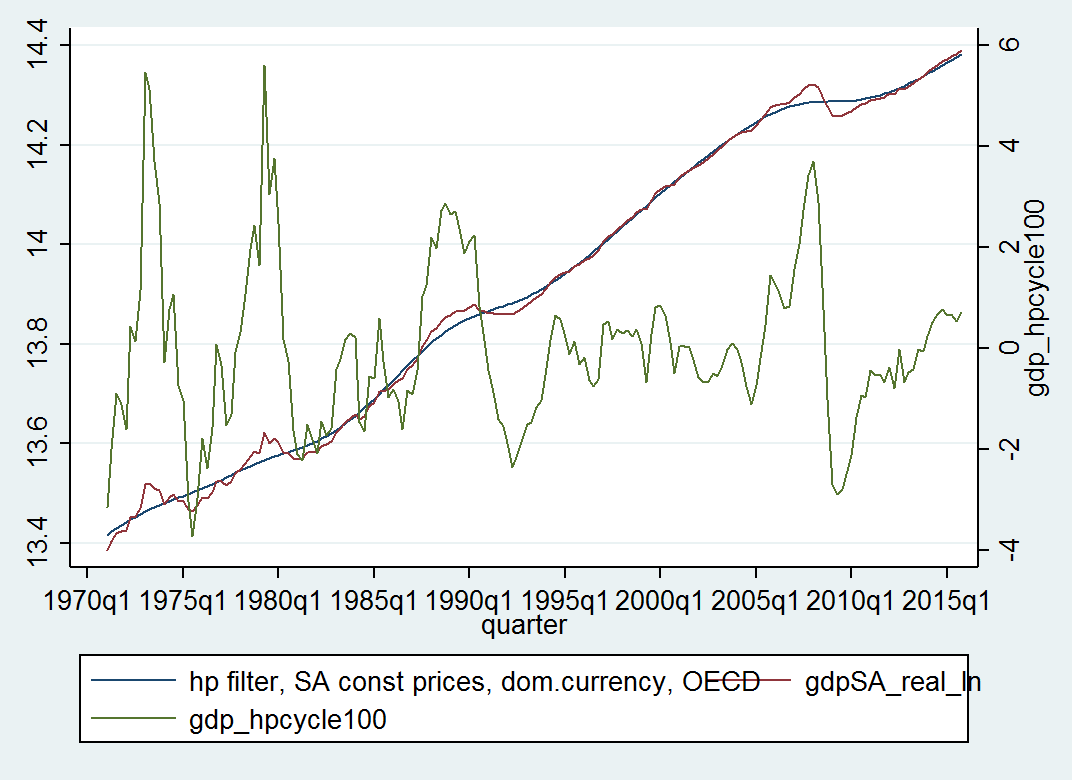
\includegraphics[trim=0 140 0 0,clip,width=0.75\columnwidth]{FIGURES/8_UKoutputDecomp}
\vspace{0.5mm}
%[trim=left bottom right top
\begin{minipage}{1.0\columnwidth}
\small	
\textbf{Note.} Decomposition of real GDP in the United Kingdom (in logarithm), 1970Q1 - 2018Q4. Blue line (left axis) is the trend estimated by Hodrick-Prescott (HP) filter. Green line (right axis) is the cycle, i.e. difference of actual GDP and estimated trend. Source: OECD.
\end{minipage}
  \end{center}

\end{frame}
\section{Aggregate Demand}
\begin{frame}{Outline}
\tableofcontents[currentsection]
\end{frame}
%---FRAME------------------------------------------------------------------------------
%---FRAME------------------------------------------------------------------------------
%\subsection{AS-AD}
%---FRAME------------------------------------------------------------------------------
%\begin{frame}
%\frametitle{Outline}
%\tableofcontents[currentsubsection]
%\end{frame}
%---FRAME------------------------------------------------------------------------------
%\begin{frame}{AS-AD}
%
%
%%\tb{Overview}
%%\begin{itemize}
%%\small
%%\item Monetary policy: exogenous
%%\item Exchange rate: endogenous
%%\end{itemize}
%
%\medskip
%\tb{Steps of our analysis}
%\begin{mytemize}
%\small
%\item \emph{How does aggregate demand work?}
%\begin{itemize}
%\small
%\item Natural rate of interest
%\item AD in the long run
%\item AD in the short run
%\end{itemize}
%\item The complete system
%\begin{itemize}
%\small 
%\item short run
%\item medium run
%\item long run
%\end{itemize}
%\item Policy example: Monetary policy
%\end{mytemize}
%
%
%\end{frame}
%---FRAME------------------------------------------------------------------------------
\begin{frame}{Aggregate Demand}
    A macroeconomic relationship between \textbf{inflation} (or price level$^*$) and \textbf{GDP} describing the Keynesian IS-TR or IS-TR-IFM equilibrium. We will plot it in $(Y, \pi)$ space.
    \\ \vfill

    \tr{Aggregate Demand $\neq$ sum of agents' demands for goods !!} \\
    \vfill
    AD is a \textbf{negative} relationship between $Y$ and $\pi$ in the 3 settings that we have seen: closed economy, fixed exchange rate economy, flexible exchange rate economy. The \textbf{reason} for the negative relationship is \textbf{different} in the 3 cases \\
\vfill
    $^*$: AD in $(Y, P)$ space is derived from the IS-LM model
\end{frame}

\begin{frame}{Aggregate Demand in a closed economy}
  A closed-economy AD is obtained from IS-TR model with \textbf{TR that reacts to inflation}:
	$$i = \bar i + \textcolor{red}{a(\pi - \bar \pi)} + b\left(\frac{Y- \bar Y}{\bar Y}\right)$$

  When solving the IS-TR model, one can eliminate $i$ and obtain $Y$ as a function of $\pi$ \textcolor{mint}{-- try this at home} \\
  \vfill
  We will construct the AD curve graphically, as we did for IS
  
\end{frame}



%---FRAME------------------------------------------------------------------------------
%---FRAME------------------------------------------------------------------------------
\begin{frame}{AD curve construction}

\begin{columns}
\column{0.5\linewidth}
Assume an increase in $\pi$:
\begin{itemize}
  \item Central bank reacts by raising interest rates for whatever $Y$: \textbf{shift} of TR 
\item $i\uparrow$ \rarr $I \downarrow$ movement \textbf{along IS} to the left
\item In the $(Y, \pi)$ space, $Y$ lower for higher $\pi$: downward sloping \tb{AD}
\end{itemize}
\vfill
\textbf{Shifts in AD}
\begin{itemize}
  \item Can come from IS: any shift in desired demand
  \item Can also come from TR: $\bar i, \bar{\pi}$
%\item \emph{IFM}: $\Delta i^* \neq 0$
\end{itemize}
% COLUMN(2)
\column{0.45\linewidth}
\vspace{7cm}
 AD \& IS-TR:
%\centering
%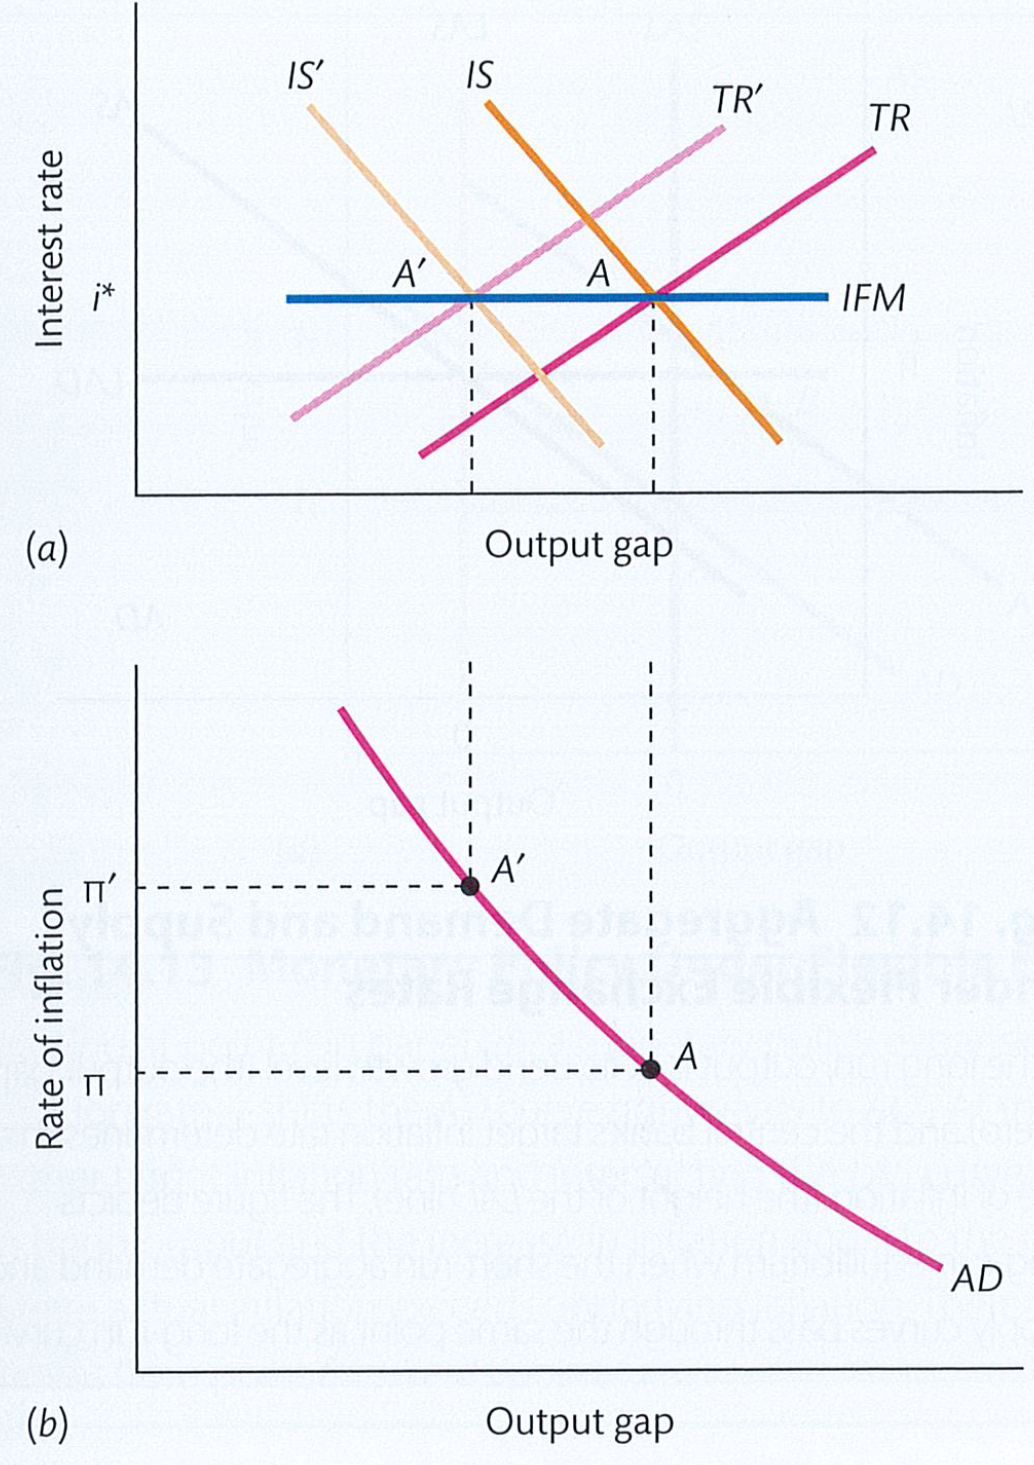
\includegraphics[clip,width=1.1\columnwidth]{FIGURES/9_ASAD_Flexible_shortrun}
%%\vspace{-2mm}
%
%\begin{minipage}{1.0\columnwidth}
%\tiny	
%%	\textbf{Note.} The Figure shows the average behaviour of variables around cyclical peaks in eight countries.\\
%\textbf{Source.} Burda and Wyplosz (2017), Figure 14.11.\\
%\end{minipage}
	
\end{columns} 	 

\end{frame}


%---FRAME------------------------------------------------------------------------------
%\subsection{How to Use the AS-AD Framework}
%---FRAME------------------------------------------------------------------------------
%\begin{frame}
%\frametitle{Outline}
%\tableofcontents[currentsubsection]
%\end{frame}
%---FRAME------------------------------------------------------------------------------
\begin{frame}{Shocks shifting AD: government spending}
  \vspace{-3cm}
 \small \textbf{Positive fiscal policy shock}, $\bar{G}'> \bar{G}$
 \vfill
\end{frame}

\begin{frame}{Shocks shifting AD: monetary policy}
  \vspace{-3cm}
 \small \textbf{Higher natural interest rate}, $\bar{i}'> \bar{i}$
 \vfill
%\begin{center}
%%{\footnotesize
%%Figure. Exchange rate of Danish krona vis-a-vis (a) EUR and (b) USD  \\
%%}
%%\vspace{-2mm}
%\begin{figure}[h!]
%%\caption{Figure. Net}
%	\subfigure{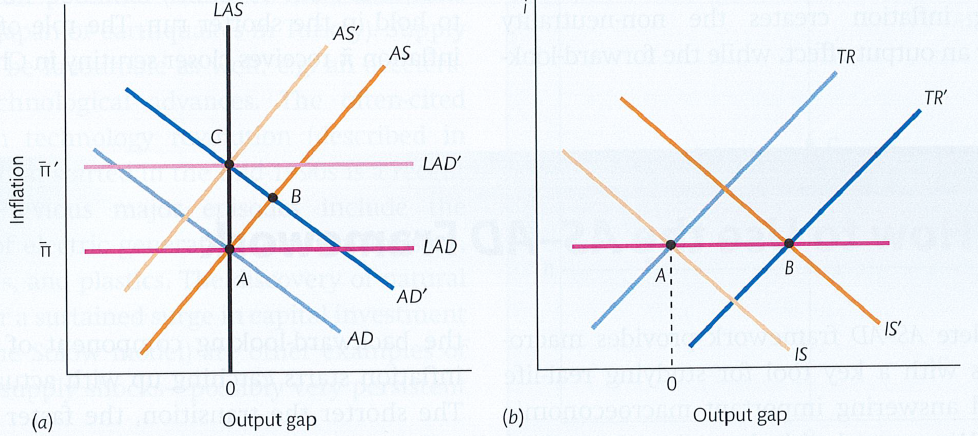
\includegraphics[trim=0 0 0 0,clip,width=0.85\textwidth]{FIGURES/9_ASAD_FlexibleMP}
%	}      
%	%} 		
%%	\label{fig:GPD} 
%	%[trim=left bottom right top
%\end{figure}
%%\vspace{-2mm}
%\begin{minipage}{0.5\columnwidth}
%\tiny	
%%\textbf{Note.} Inflation in Denmark and the euro area (1992-2016).  
%\textbf{Source.} Burda \& Wyplosz (2017), Figure 14.13.\\
%\end{minipage}
%\end{center}
\end{frame}


\begin{frame}{Open economy AD: Inflation \& real exchange rate}
Real exchange rate formula: $\sigma = \frac{S P}{P^*}$ \\
\vfill
What is a formula for a \textbf{change} of $\sigma$? \\
\vfill
To study changes, take logarithm of both sides and apply the total differential: 
$$\ln \sigma = \ln S + \ln P - \ln P^*$$
$$\frac{d \sigma}{\sigma} = \frac{d S}{S} + \frac{d P}{P}  - \frac{d P^*}{P^*} $$
$$\frac{d \sigma}{\sigma} = \frac{d S}{S} + \pi  - \pi^* $$
  
  
\end{frame}




\begin{frame}{AD construction: fixed exchange rate regime}
\begin{columns}
\column{0.5\linewidth}
\begin{itemize}
\item Assuming $\pi\uparrow$
\item $\frac{d \sigma}{\sigma} = \frac{d S}{S} + \pi  - \pi^* = \pi - \pi^*$ \rarr $\sigma\uparrow$
\item IS-(TR)-IFM: IS shifts to the left, intersection with IFM has lower $Y$
\item[\rarr] inflation higher, output lower: downward sloping \tb{AD}
\end{itemize}
\textbf{Shifts in AD}
\begin{itemize}
  \item Demand shocks (IS)
  \item Devaluations, revaluations ($\bar S$)
  \item IFM ($i^*$) 
\end{itemize}
% COLUMN(2)
\column{0.45\linewidth}

%\centering
%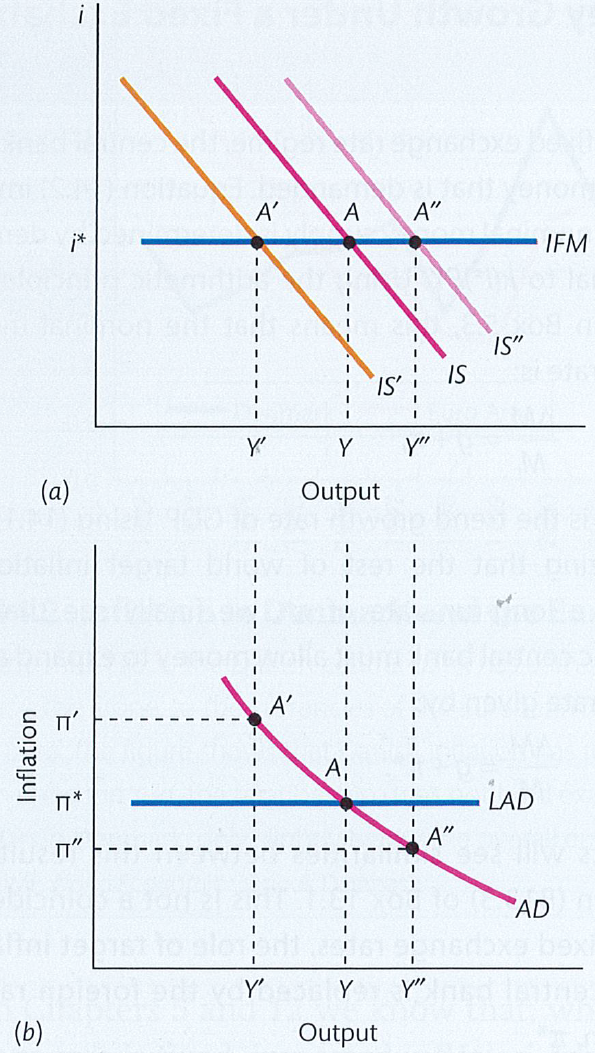
\includegraphics[clip,width=1\columnwidth]{FIGURES/9_AD_FixedFX}
%%\vspace{-2mm}
%
%\begin{minipage}{1.0\columnwidth}
%\tiny	
%%	\textbf{Note.} The Figure shows the average behaviour of variables around cyclical peaks in eight countries.\\
%\textbf{Source.} Burda and Wyplosz (2017), Figure 14.11.\\
%\end{minipage}
	
\end{columns} 	 
\end{frame}

%\begin{frame}{AD-AS with fixed exchange rate regime}
%  \vspace{-5cm}
%  New mechanism: long-run convergence of $\pi$ to $\pi^*$ through changes of $\sigma$.
%\end{frame}

%\begin{frame}{%
%\protect\hypertarget{flexible-exchange-rate-ad}{%
%LAD under flexible exchange rate}}
%
%\begin{mytemize}
% 
%\item
%  LAD: Taylor rule enforces \(\pi = \bar \pi\) in long run, as in closed economy
%  \item \tr{Different} from \tr{fixed} exchange rate regime, where LAD is $\pi = \pi^*$
%\end{mytemize}
%
%\end{frame}

\begin{frame}{AD construction: flexible exchange rate regime}
\begin{columns}
\column{0.5\linewidth}
\begin{itemize}
\item Assuming $\pi\uparrow$
\item TR shifts up (as in closed economy) \rarr IS-IFM intersection with lower $Y$
\item IS moves left to the TR-IFM intersection because $\frac{d \sigma}{\sigma} = \frac{d S}{S} + \pi  - \pi^*$ \rarr $\sigma\uparrow$
\item[\rarr] inflation higher, output lower: downward sloping 
\tb{AD}
\end{itemize}
\textbf{Shifts in AD}
\begin{itemize}
  \item TR shocks ($\bar i, \bar \pi$)
  \item IFM ($i^*$) -- opposite effect to fixed exchange rate case
  \item \tr{NOT} the demand shocks (IS shifters other than $\sigma$) 
\end{itemize}
% COLUMN(2)
\column{0.45\linewidth}

%\centering
%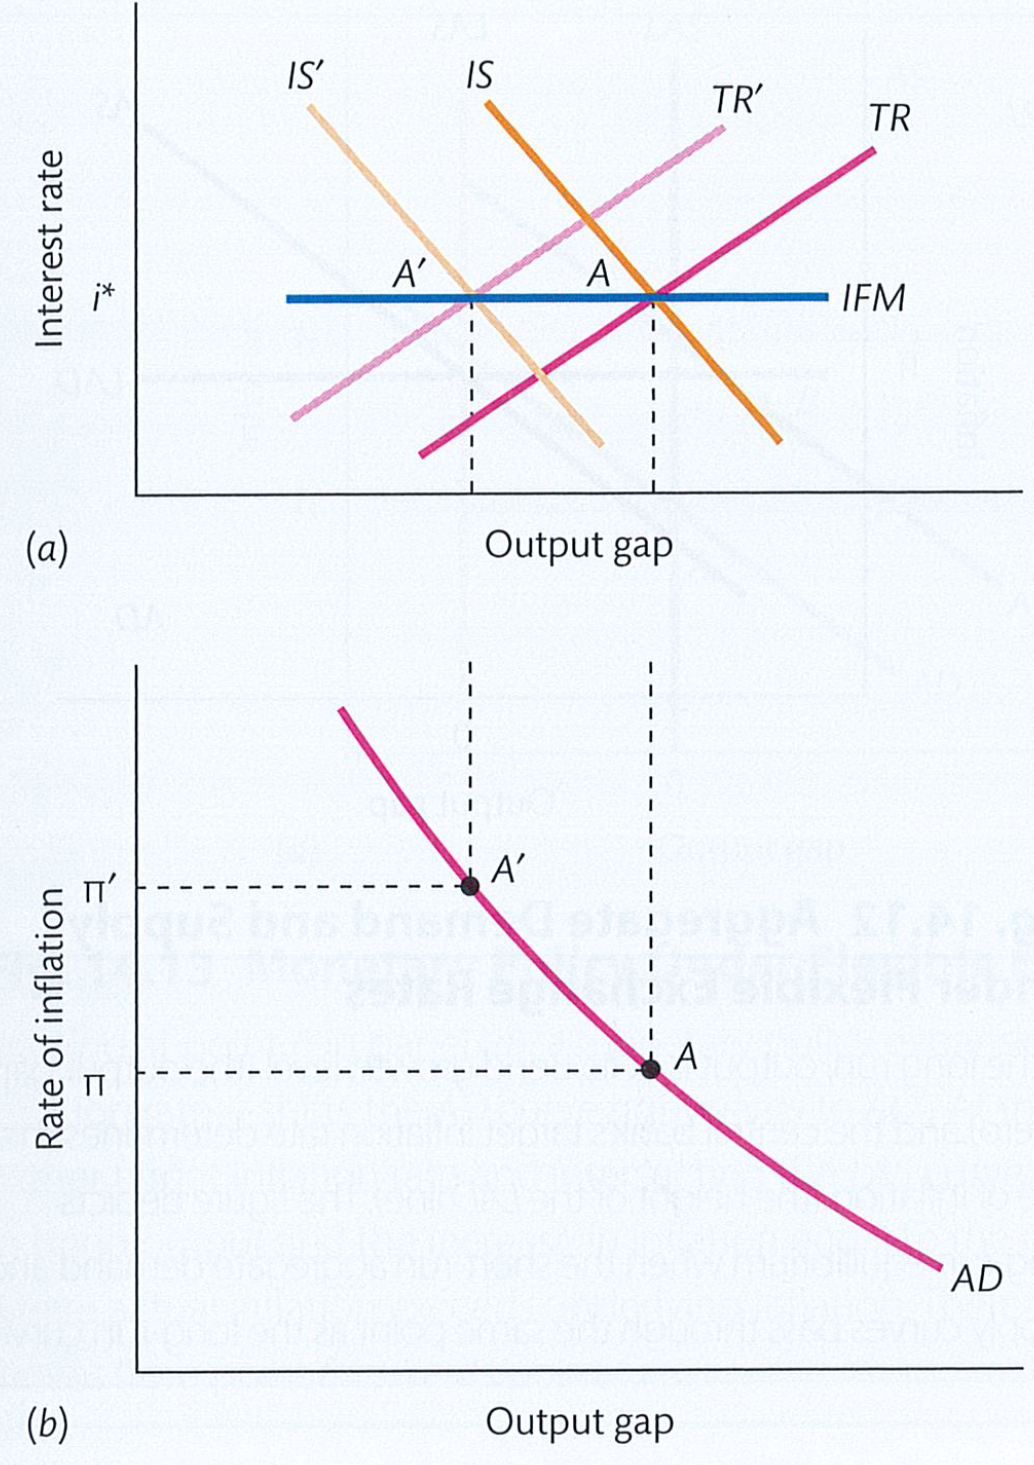
\includegraphics[clip,width=1\columnwidth]{FIGURES/9_ASAD_Flexible_shortrun.png}
%%\vspace{-2mm}
%
%\begin{minipage}{1.0\columnwidth}
%\tiny	
%%	\textbf{Note.} The Figure shows the average behaviour of variables around cyclical peaks in eight countries.\\
%\textbf{Source.} Burda and Wyplosz (2017), Figure 14.11.\\
%\end{minipage}
	
\end{columns} 	 
\end{frame}


%---FRAME------------------------------------------------------------------------------
%\begin{frame}{Empirical evidence for non-neutrality?}
%
%\begin{itemize}
%\small
%\item We have split our analysis in three time horizons: \tb{short, medium and long run}. What do they mean in practice?
%\begin{itemize}
%\small
%\item \emph{Short run}: one to two years
%\item \emph{Medium run}: two to five years
%\item \emph{Long run}: beyond 5 years
%\end{itemize}
%\end{itemize}
%
%%\frametitle{Evidence of monetary policy non neutralities}
%
%\begin{center}
%{\small
%Figure. Estimated dynamic response to monetary policy shock
%}
%\end{center}
%\vspace{-2mm}
%\begin{figure}
%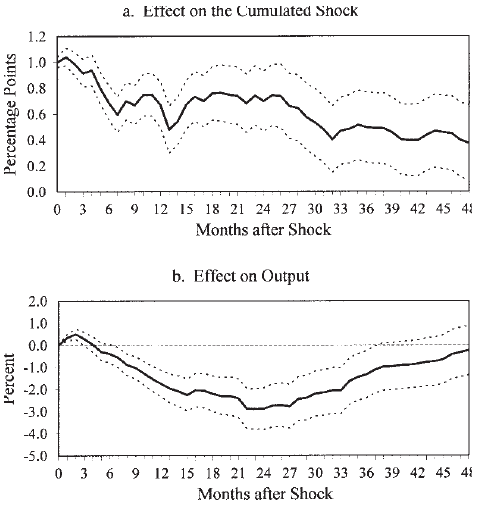
\includegraphics[width=0.4\textwidth]{FIGURES/RomerRomerFig9_ab}
%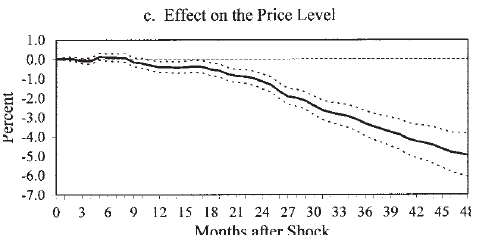
\includegraphics[width=0.4\textwidth]{FIGURES/RomerRomerFig9_c}
%\end{figure}
%\begin{minipage}{0.99\columnwidth}
%\tiny	
%\textbf{Note.} The effects of a (US) monetary policy shock in a VAR model. The authors use a narrative approach for the construction of monetary policy shocks. \emph{Source:} Romer \& Romer (2004), Figure 9.
%\end{minipage}
%
%
%\end{frame}
%%---FRAME-----------------------------------------------------
%\begin{frame}{Further evidence of monetary policy non neutrality}
%
%\begin{center}
%{\small
%Figure. Estimated dynamic response to monetary policy shock
%}
%\end{center}
%\begin{figure}
%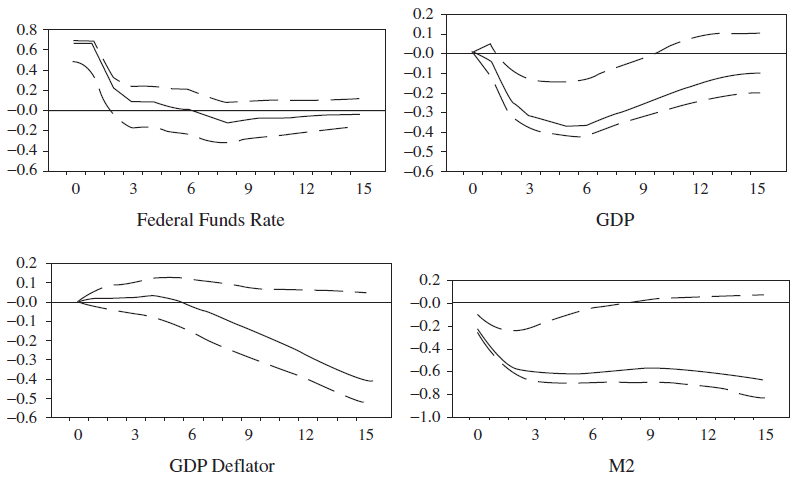
\includegraphics[width=0.75\textwidth]{FIGURES/CEE1999}
%\end{figure}
%\begin{minipage}{0.99\columnwidth}
%\tiny	
%\textbf{Notes.} The effects of a (US) monetary policy shock in a VAR model, frequency is a quarter. Depending on the identifying assumptions, the results might vary substantially. \emph{Source:} Christiano, Eichenbaum and Evans (1999), as shown in Gali (2008), Figure 1.1.
%\end{minipage}
%
%
%
%\end{frame}
%---FRAME------------------------------------------------------------------------------
%\begin{frame}{Medium-run AD: Natural rate of interest}
%  \begin{mytemize}
%	\item In the long run, central bank assumed to set interest such that $\pi = \bar \pi$ for whatever $Y$ (which is $\bar Y$ anyways) 
%	\begin{mytemize}
%	\item horizontal \tb{LAD}
%	\item will become more relevant in open economy analysis
%	\end{mytemize}
%  \end{mytemize}
%\begin{center}
%%{\footnotesize
%%Figure. Exchange rate of Danish krona vis-a-vis (a) EUR and (b) USD  \\
%%}
%%\vspace{-2mm}
%\begin{figure}[h!]
%%\caption{Figure. Net}
%	\subfigure{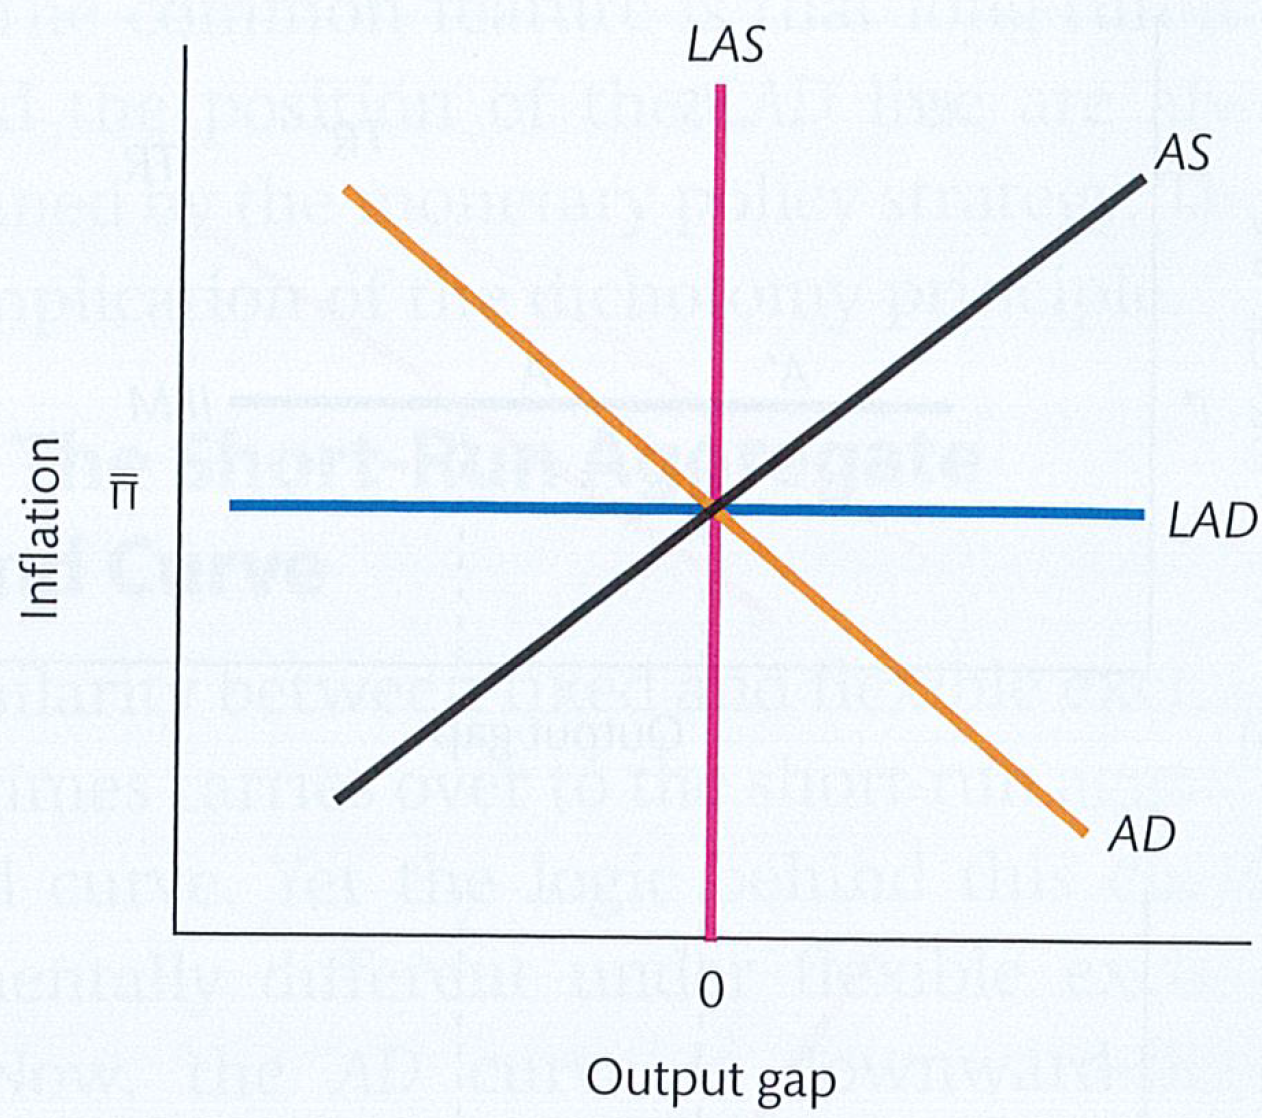
\includegraphics[trim=0 0 0 0,clip,width=0.45\textwidth]{FIGURES/9_ASAD_Flexible}
%	}      
%	%} 		
%%	\label{fig:GPD} 
%	%[trim=left bottom right top
%\end{figure}
%%\vspace{-2mm}
%\begin{minipage}{0.5\columnwidth}
%\tiny	
%%\textbf{Note.} Inflation in Denmark and the euro area (1992-2016).  
%\textbf{Source.} Burda \& Wyplosz (2017), Figure 14.12.\\
%\end{minipage}
%\end{center}
%\end{frame}
%\section{Supply side}
%\subsection{Long run supply (Flexible Prices)}
%\begin{frame}{Supply-determined output in the long run}
%
%\begin{columns}
%
%\column{0.65\linewidth}
%\begin{itemize}
%\item What determines output in the \textbf{long run (on the trend)}?
%\item A simplistic production function:
%\begin{itemize}
%\item Only labor ($L$) used for production, $Y =F(L)$
%\item $L$'s \tb{marginal product} $=$ \tb{real wage} \rarr equilibrium $\bar L$, output $\bar Y$
%\end{itemize}
%\item What about demand? 
%  \begin{itemize}
%	\item In the medium run, \textbf{demand adjusts to supply} via \tb{real wage}
%  \end{itemize}
%\end{itemize}
%
%% COLUMN(2)
%\column{0.35\linewidth}
%
%\centering
%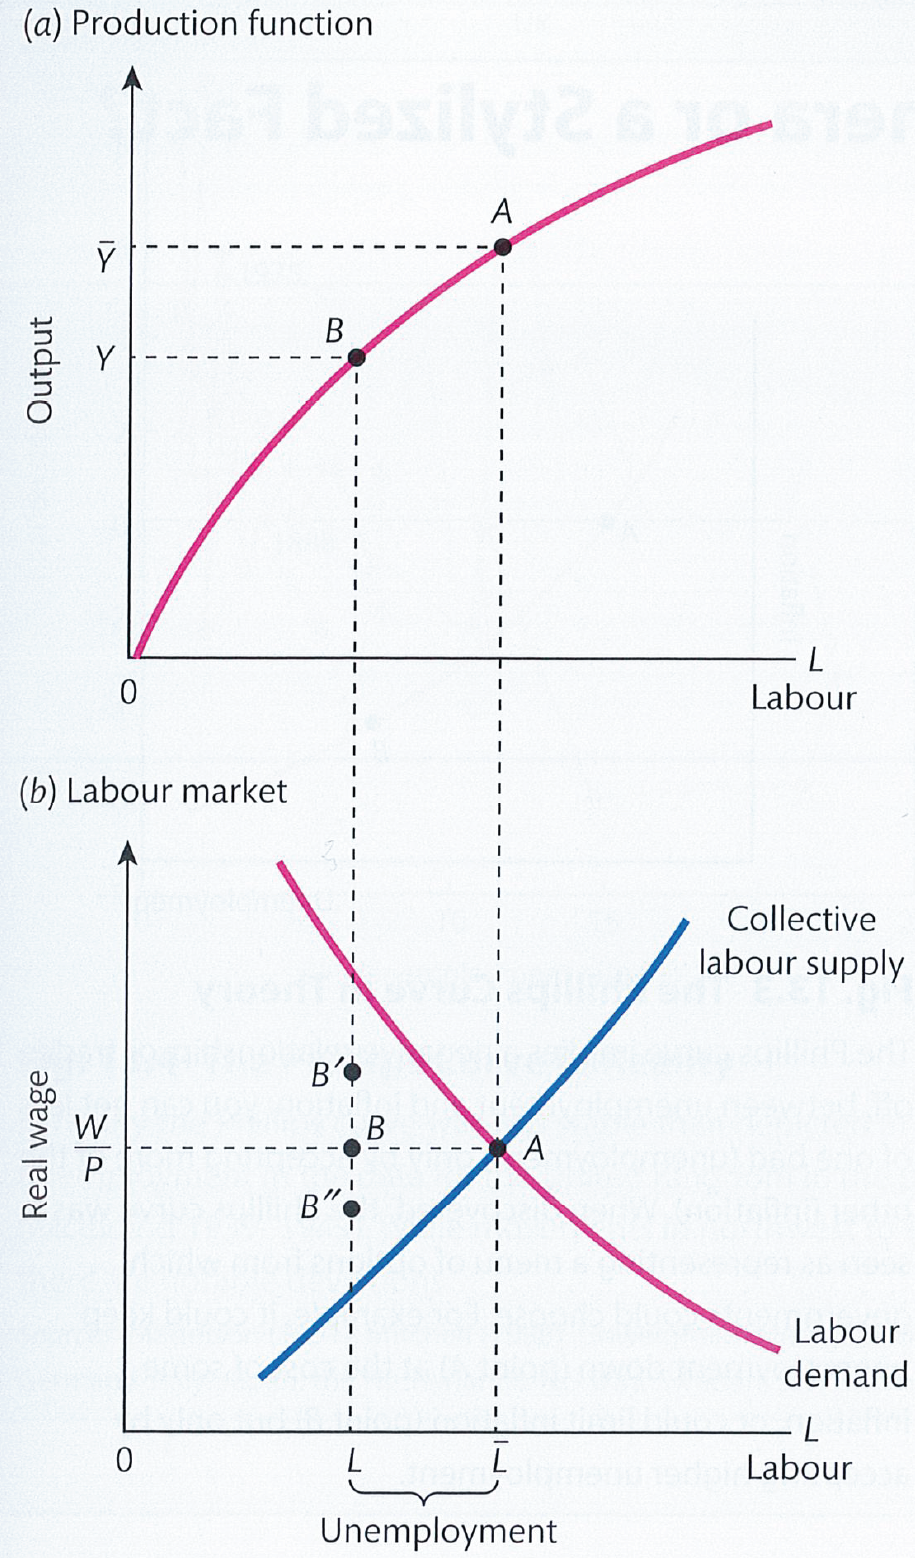
\includegraphics[clip,width=1.1\columnwidth]{FIGURES/8_LongRun}
%%\vspace{-2mm}
%
%\begin{minipage}{1.0\columnwidth}
%\tiny	
%%	\textbf{Note.} The Figure shows the average behaviour of variables around cyclical peaks in eight countries.\\
%\textbf{Source.} Burda and Wyplosz (2017), Figure 13.2.\\
%\end{minipage}
%	
%\end{columns} 	       
%
%\end{frame}







%---FRAME------------------------------------------------------------------------------
%\begin{frame}{Supply-determined output in the long run}
%
%\emph{Principle of adjustment process:} \\
%
%\medskip
%
%\tb{$\Rightarrow$ Prices rise when demand for goods is strong, and fall when demand is weak.}
%
%\medskip
%
%\begin{itemize}
%\small
%\item assumption: flexible prices, 'sticky' wages
%\item reduction in prices $+$ sticky wages $=$ real wage W/P $\uparrow$, (point $B'$)
%\item over time $W\downarrow$, and $W/P \downarrow$
%\item from $IS-TR$ curves, central bank will lower $i$ when $P\downarrow$
%\item investment $\uparrow$
%%\item real exchange rate effect, $SP/P^*\downarrow$ (\emph{depreciation}), $NX\uparrow$
%\item $\rightarrow$ demand goes up $Y\uparrow$ 
%\item ...convergence back to point $A$ %(however, lower real wage!)
%\end{itemize}
%
%\end{frame}
%---FRAME------------------------------------------------------------------------------
%\begin{frame}{From the short run to the long run}
%
%\begin{itemize}
%\small
%\item How to reconcile the two diametrically opposite assumptions?
%\item $\Rightarrow$ intellectual debate lead to the \emph{New Keynesian synthesis}
%\item Assume an \tb{expansion of money supply}: transition
%\end{itemize}
%
%\begin{center}
%%{\small
%%Figure. 
%%}
%
%%\vspace{-2mm}
%\begin{figure}[h!]
%	\subfigure{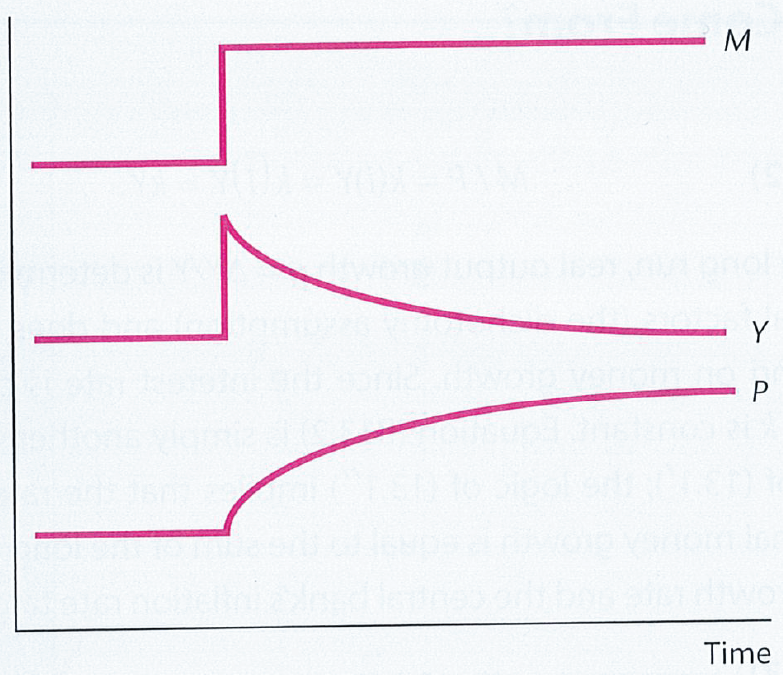
\includegraphics[trim=0 0 0 0,clip,width=0.5\textwidth]{FIGURES/8_ShortLongRun}
%	}      
%	%\subfigure{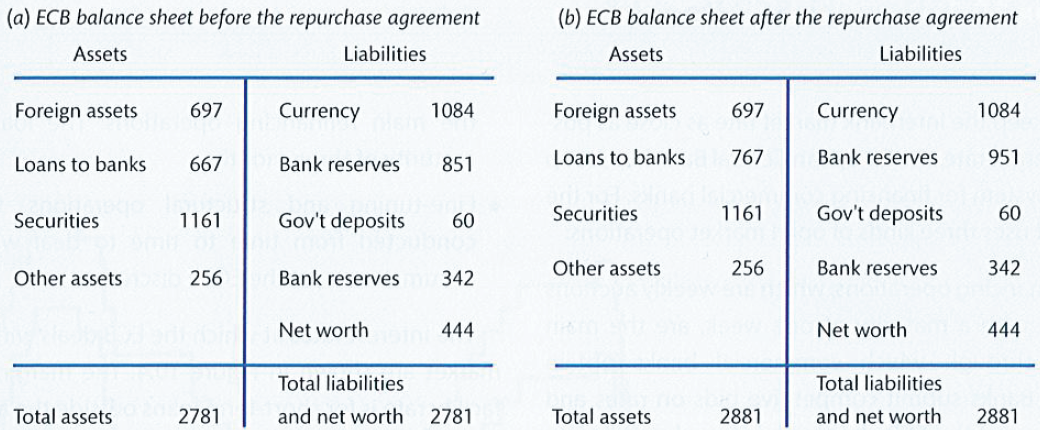
\includegraphics[trim=0 00 0 00,clip,width=0.6\textwidth]{FIGURES/5_CB_balance_sheet_OMO}
%	%} 	
%	%[trim=left bottom right top
%\end{figure}
%%\vspace{-2mm}
%\begin{minipage}{0.5\columnwidth}
%\tiny	
%\textbf{Source.} Burda and Wyplosz (2017), Figure 13.1.\\
%\end{minipage}
%\end{center}
%\end{frame}
%---FRAME------------------------------------------------------------------------------

%\subsection{The Phillips Curve}
%---FRAME------------------------------------------------------------------------------

%---FRAME------------------------------------------------------------------------------
\section{Medium run aggregate supply}
%\begin{frame}
%\frametitle{Outline}
%\tableofcontents[currentsubsection]
%\end{frame}
%\begin{frame}{Medium run: Phillips Curve and Okun's law}
%\begin{mytemize}
%\item Keynesian theory: no relation between aggregate output and inflation --- the \emph{missing equation} problem
%\item Two empirical findings used to fill the theory gap:
%  \begin{mynumerate}
%	\item A. W. Phillips (1958): negative correlation between wage inflation and unemployment rate
%	\item A. Okun (1962): negative correlation between unemployment rate and GDP changes
%  \end{mynumerate}
%\item[\rarr] inflation-output relationship
%\end{mytemize}
%\end{frame}
%---FRAME------------------------------------------------------------------------------
\begin{frame}{Supply side in the medium run: theory}
    Main idea: firms that have some 
    \tb{market power} \rarr can set prices \\
    \vfill 
    Important factors for price setting:
    \begin{mynumerate}
        \item \tb{Marginal cost} (we consider \tb{labor cost} only)
        \item \tb{Expected aggregate price level in the future}: prices are not perfectly flexible in medium run \rarr price chosen today may remain for a while, must be adequate for future conditions
    \end{mynumerate}

\vfill
Both \tb{Phillips Curve (PC)} and \tb{Aggregate Supply (AS)} relate positively \textbf{current inflation} to \textbf{expected inflation}. In addition, PC relates negatively inflation to \textbf{unemployment}, while AS relates positively inflation to \textbf{output}
\end{frame}



\begin{frame}{The Phillips Curve}
\begin{center}
%{\small
%Figure. 
%}
A regularity in the UK data... \hspace{10mm} ...transformed into a theory
%\vspace{-2mm}
\begin{figure}[h!]
	\subfigure{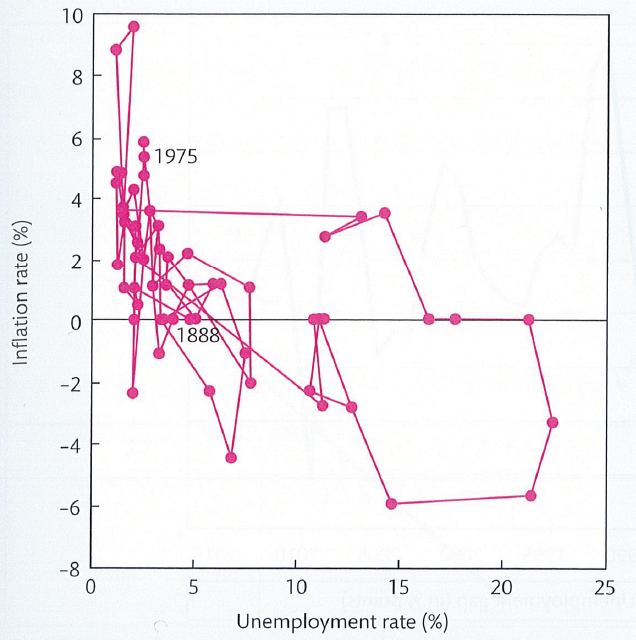
\includegraphics[trim=0 00 0 00,clip,width=0.45\textwidth]{FIGURES/8_PCdataUK}
	} 	
 \subfigure{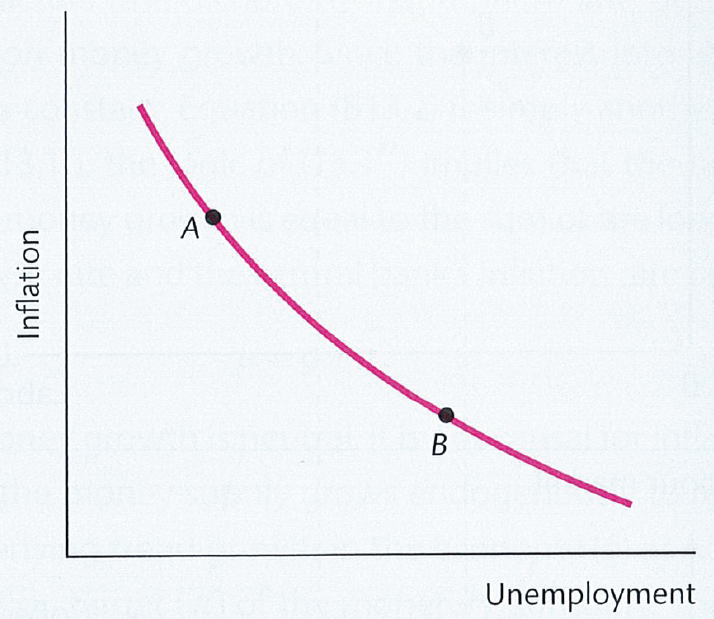
\includegraphics[trim=0 0 0 0,clip,width=0.45\textwidth]{FIGURES/8_PCtheory}
	}      
	%[trim=left bottom right top
\end{figure}
%\vspace{-2mm}
\begin{minipage}{1.0\columnwidth}
\centering
\tiny
\textbf{Source.} Burda and Wyplosz (2017), Figure 13.3, Figure 13.4.\\
\end{minipage}
\end{center}

\end{frame}
%---FRAME------------------------------------------------------------------------------
\begin{frame}{Supply side of inflation: price setting}
\begin{mytemize}
    \item Firms produce goods with labor and have market power on both goods market and labor market
    \item[\rarr] Prices depend marginal cost (wage) and \tb{demand elasticity}
    \item Prices are \tb{sticky}: price set today can remain in the future
    \item[\rarr] The price choice takes into account which prices other firms may charge in the future \rarr \textbf{expected inflation matters}
\end{mytemize}
\vfill
How are prices linked to unemployment ($u$)? In an expansion ($Y > \bar Y$), $u$ is low, and incomes relatively high \rarr demand elasticity of consumers is lower \rarr firms can charge higher prices
\end{frame}

\begin{frame}{Suppy side of inflation: labor market}
Labor market strengthens the link of current prices to future inflation and to unemployment: 
   \begin{mytemize}
        \item Consider \tb{wage bargaining} between firms and workers/ unions
        \item Wages stay fixed until next negociation \rarr inflation may erode real income \rarr current wage negotiation must be based on \textbf{expected inflation} 
        \item In an expansion ($Y > \bar Y$, low $u$) workers have higher bargaining power (less afraid to lose jobs) and some may work overtime \rarr wages rise
        \item[\rarr] firms' marginal cost (wage) and price depend:
        \begin{mynumerate}
            \item positively on $\pi^e$
            \item negatively on $u$
        \end{mynumerate}
   \end{mytemize} 
\end{frame}

\begin{frame}{Theoretical Phillips Curve}
   The factors influencing firms' optimal price also influence current inflation \\
   \vfill
   
   One gets the theoretical Phillips Curve:
   $$\pi = b \cdot u^{gap} + \pi^e + s$$
   Where 
   \begin{mytemize}
       \item $u^{gap} = u - \bar u$ and $\bar u$ is \tb{natural unemployment} rate: seasonal, job-to-job transitions...
       \item $b<0$
       \item $s$ is a \tb{supply shock}: a variable regrouping all non-wage macroeconomic factors that raise firms' marginal cost
   \end{mytemize}
   \vfill
   Typical supply shock -- energy prices
\end{frame}
%\begin{frame}{The Phillips Curve: policy trade-off}
%
%
%\begin{mytemize}
%\item Phillips curve as an intuitive and practical idea for policy-makers: cannot achieve all good macro indicators at once:
%  \begin{mytemize}
%\item Either lower inflation and higher unemployemt, ...
%\item ... or higher inflation, but lower unemployment.
%  \end{mytemize}
%\item Slope of Phillips curve referred to as \tb{sacrifice ratio}
%\end{mytemize}
%
%\medskip
%
%\medskip
%
%\emph{"I would rather prefer 5\% inflation, then 5\% unemployment (...)"}
%\flushright{Helmut Schmidt, 1978}
%
%\end{frame}
%---FRAME------------------------------------------------------------------------------
%\begin{frame}{Okun's Law}
%
%\begin{itemize}
%\small
%\item \emph{Missing element:} Aggregate relationship between output and inflation
%\end{itemize}
%\begin{align*}
%\text{\alert{inflation}} \underset{(1)PC}{\quad \leftarrow \rightarrow \quad} \text{unemployment} \underset{(2)OL}{\quad \leftarrow \rightarrow \quad} \text{\alert{output}}
%\end{align*}
%
%\begin{mynumerate}
%\small
%\item (1)\tb{Phillips curve} (PC) not sufficient
%\item (2)\tb{Okun's Law} (OL), Arthur Okun (1928-1980):
%\begin{itemize}
%\small
%\item negative relationship between output and unemployment.
%\end{itemize}
%\end{mynumerate}
%
%
%\end{frame}
%---FRAME------------------------------------------------------------------------------
\begin{frame}{From $u$ to $Y$ -- Okun's Law, AS}

Data shows strong negative relationship between unemployment gap $u -\bar u$ and output gap $(Y-\bar Y)/\bar{Y}$: \tb{Okun's law} \\
\vfill
\rarr Can replace $u^{gap}$ in Phillips Curve with $Y^{gap}$ \\
\vfill
\begin{mytemize}
\item \tb{AS} relationship $\pi = a \cdot Y^{gap} + \pi^e + s$, with $a > 0$
\end{mytemize}

\begin{center}
%\vspace{-2mm}
\begin{figure}[h!]
%	\subfigure{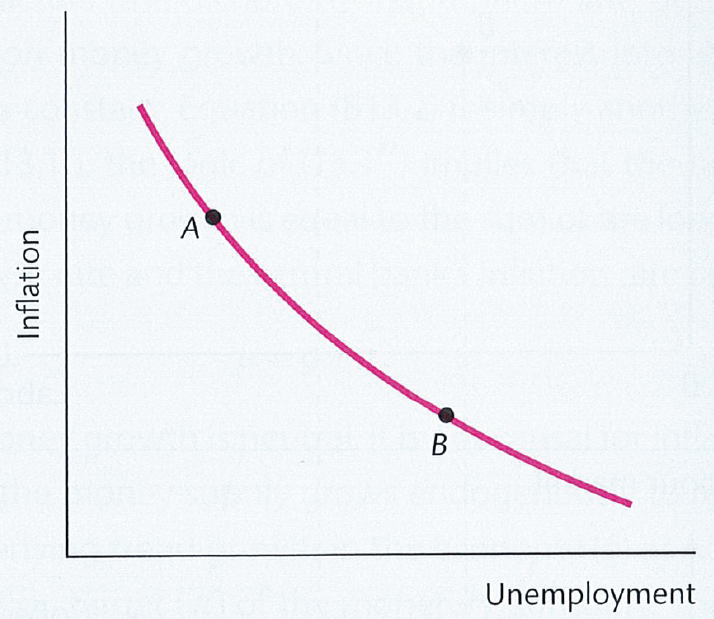
\includegraphics[trim=0 0 0 0,clip,width=0.45\textwidth]{FIGURES/8_PCtheory}
%	}      
	\subfigure{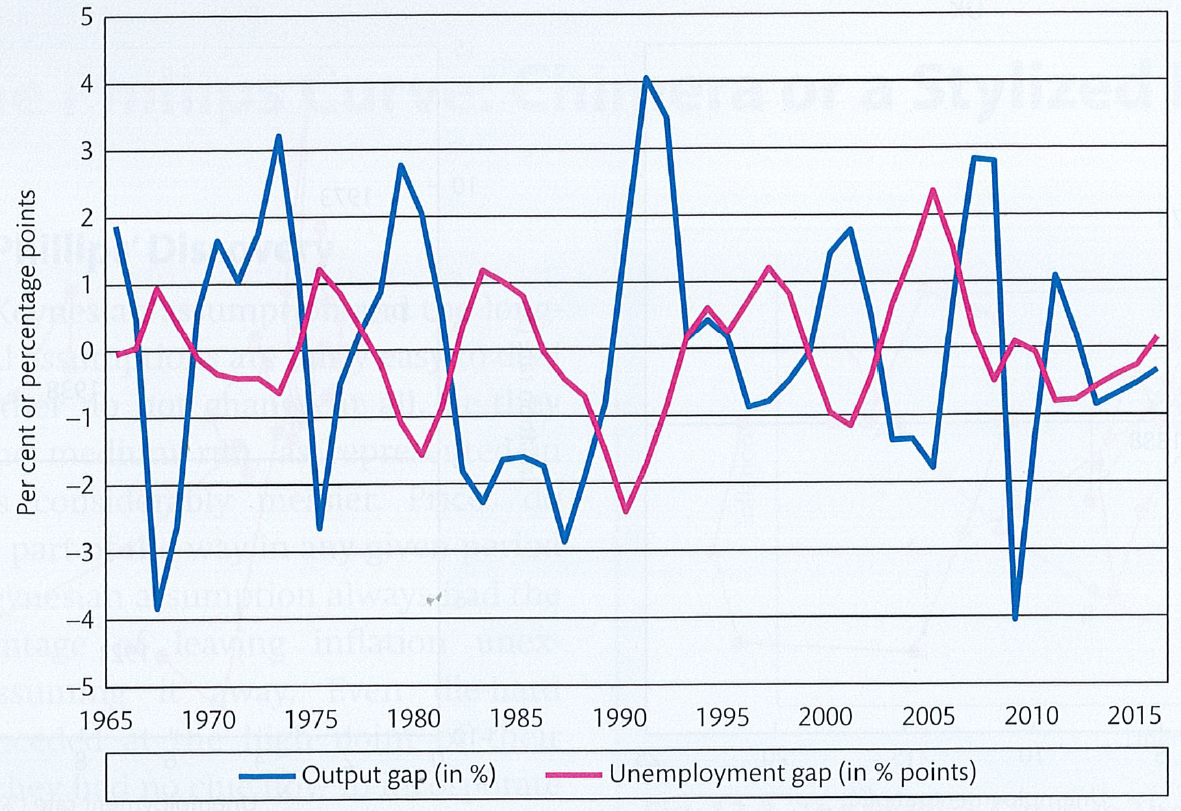
\includegraphics[trim=0 00 0 00,clip,width=0.65\textwidth]{FIGURES/8_OkunsLawDE}
	} 	
	%[trim=left bottom right top
\end{figure}
%\vspace{-2mm}
\begin{minipage}{0.97\columnwidth}
\tiny	
The output and unemployment gap in Germany, 1970-2016. \textbf{Source.} Burda and Wyplosz (2017), Figure 13.5.\\
\end{minipage}
\end{center}

\end{frame}

\begin{frame}{AS and Phillips curve: symmetry}
\begin{align}
\pi =& a \cdot Y^{gap} + \pi^e + s \tag{AS} \\
  \pi =& b \cdot u^{gap} + \pi^e + s \tag{Phillips Curve}
\end{align}
  \begin{center}
%{\small
%Figure. The output gap and unemployment in Germany, 1970-2016
%}
%\vspace{-2mm}
\begin{figure}[h!]
%	\subfigure{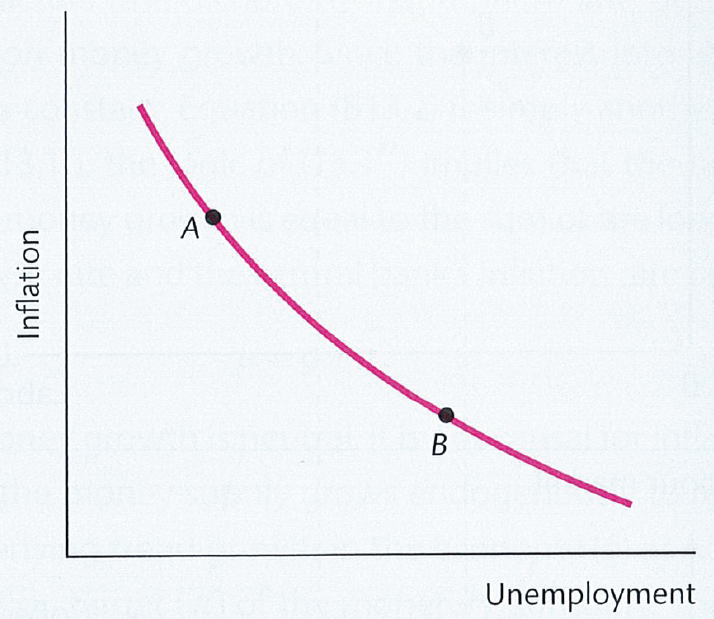
\includegraphics[trim=0 0 0 0,clip,width=0.45\textwidth]{FIGURES/8_PCtheory}
%	}      
	\subfigure{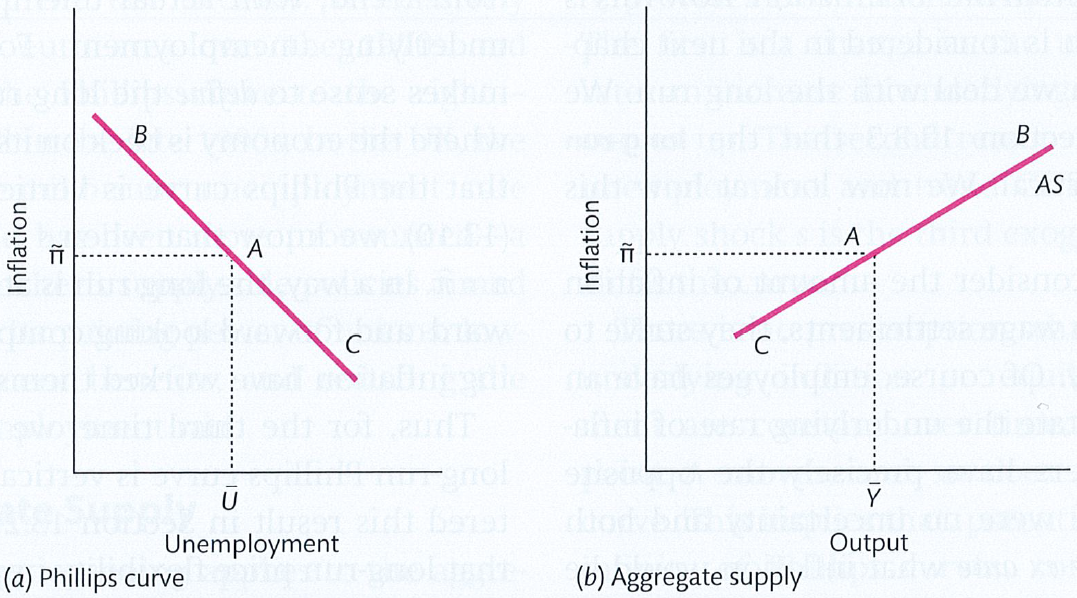
\includegraphics[trim=0 00 0 00,clip,width=0.9\textwidth]{FIGURES/8_NewPC}
	} 	
	%[trim=left bottom right top
\end{figure}
%\vspace{-2mm}
\begin{minipage}{0.90\columnwidth}
\tiny	
Burda and Wyplosz (2017), Figure 13.12.\\
\end{minipage}
\end{center}
\end{frame}

\begin{frame}{Endogenous $\pi^e$: shifts in AS}
\vspace{-4.5
cm}
Demand and supply shocks bring \tb{unexpected changes} of inflation. \tb{Rational expectations} are assumed \rarr \\ \textbf{$\pi^e$ changes} following shocks, \textbf{AS shifts}
    
\end{frame}

\section{The long run}

\begin{frame}
\frametitle{Outline}
\tableofcontents[currentsection]
\end{frame}


\begin{frame}{Money and inflation in the long run}

  \tb{Quantity Theory of Money} describes money-output relationship:
\begin{align*}
\underbrace{M}_{money\ supply} &= \underbrace{k}_{money\ velocity}\times \underbrace{P}_{price\ level} \times \underbrace{Y}_{GDP} \\
\Leftrightarrow \quad P &= \frac{M}{kY}
\end{align*}
where money velocity $k$ measures how fast money circulates. Assuming $k$ constant, taking logarithms of both sides and a \tm{total differential}:
\begin{align*}
\ln P &= \ln M - \ln k - \ln Y \\ 
\text{total differential:} \quad  \underbrace{\frac{d P}{P}}_{=\pi} &= \underbrace{\frac{d M}{M}}_{\equiv \mu} - \underbrace{\frac{d k}{k}}_{=0} - \underbrace{\frac{d Y}{Y}}_{\equiv g} \\ 
\Leftrightarrow \pi &=  \mu - g 
\end{align*}
Where $\frac{d P}{P} = \pi \approx \frac{P(t+\Delta)-P(t)}{P(t) \Delta }$ when the time step $\Delta$ is small
\end{frame}
%---FRAME------------------------------------------------------------------------------
%\begin{frame}{Monetary policy, interest in the long run}
%
%  The long-run  inflation is the inflation target in the Taylor rule: $\bar \pi = \mu - g$. Target depends on:
%  \begin{mynumerate}
%	\item Money growth rate $\mu$, a policy variable
%	\item Trend growth rate $g$ determined (mostly) by technology and demographics
%  \end{mynumerate}
%  \vfill
%  $\pi = \bar \pi, Y = \bar Y$ in the long run, so from the TR equation:
%\begin{align*}
%i = \bar{i}+a (\pi - \bar{\pi}) + b \left(\frac{Y-\bar{Y}}{\bar{Y}} \right) = \bar i
%\end{align*}
%\vfill
%Nominal interest is at \tb{natural nominal rate} in the long run. The real interest rate in the long run: 
%\begin{align*}
%\bar r = \bar i - \bar \pi = \bar i - \mu + g
%\end{align*}
%Technology and demographics affect the real interest rate: it is high in an economy with faster trend growth.
%\end{frame}
%


\begin{frame}{Long run real exchange rate}
  Absence of \tb{arbitrage} between countries assumed in long run \rarr two versions of \tb{purchasing power parity (PPP)} condition:
  \begin{mynumerate}
  \item \tb{Absolute PPP}: $\sigma = 1 \Leftrightarrow S \cdot P  = P^*$ 
  \item \tb{Relative PPP}: $\sigma$ constant: 
	$$d \sigma = 0 \Rightarrow \frac{d \sigma}{\sigma} = \frac{d S}{S} + \frac{d P}{P}  - \frac{d P^*}{P^*} = 0$$
	$$\frac{d S}{S} = \pi^* - \pi$$
  \item[\rarr] if domestic and foreign inflation rates not equal on average, permanent nominal exchange rate appreciation/depreciation
  \end{mynumerate}
  \vfill 
  Absolute PPP implies relative PPP; the converse is not true
 % \vfill
 % Micro version of PPP -- \tr{law of one price}: each good $j$ has same price in domestic and foreign economy: $S \cdot p_j = p^*_j$ \\ Sufficient, but \textbf{not necessary} for PPP to hold.
\end{frame}

\begin{frame}{Fixed exchange rates and Purchasing Power Parity}
Under the fixed exchange rate regime, purchasing power parity implies equality of inflation rates with the rest of the world:
	$$\underbrace{\frac{d S}{S}}_{=0} + \pi  - \pi^* = 0 \Leftrightarrow \pi = \pi^*$$
  \rarr horizontal line $\pi = \pi^*$ for long-run AD-AS analysis of fixed exchange rate economies
  %\vfill
  %Most strict version -- \tr{law of one price}: each good $j$ has same price in domestic and foreign economy: $S \cdot p_j = p^*_j$ -- sufficient, but \textbf{not necessary} for PPP to hold.
\end{frame}

\begin{frame}{Change of exchange rate regime and real exchange rate: case study}
  
  \begin{figure}[ht]
	\centering
	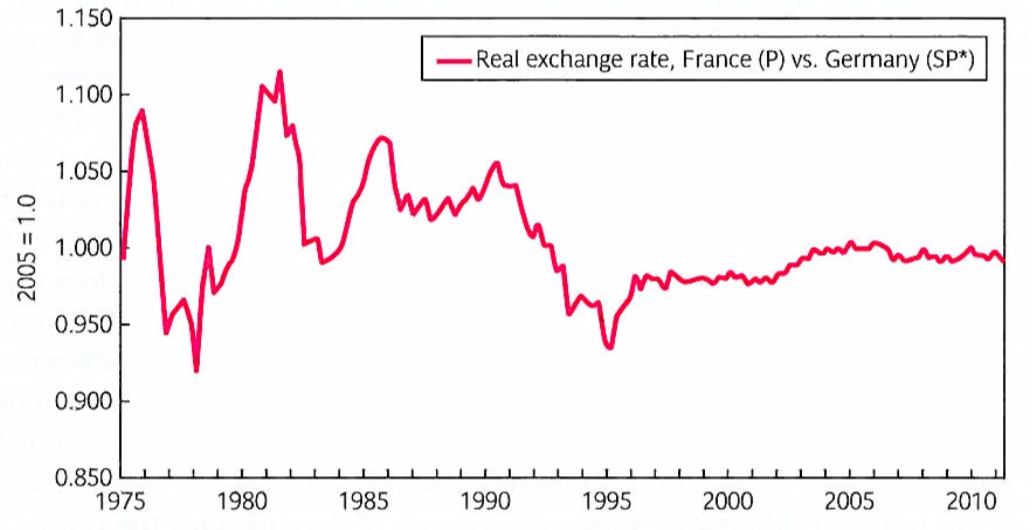
\includegraphics[width=0.95\textwidth]{FIGURES/Fig_13_9_RER_France_Germany}
 \end{figure}
 \begin{minipage}{0.6\columnwidth}
\tiny	
%\textbf{Note.} Actual examples of trajectories, extracted from the French and Italian CPI databases. The dotted lines indicate events of price changes.
\textbf{Source.} Burda and Wyplosz (2017), Figure 13.9.\\
\end{minipage}
\end{frame}

\begin{frame}{Long-run aggregate supply}
\begin{columns}
    \column{0.5\textwidth}
\tb{Rational expectations} \rarr all forecast errors are temporary \rarr $\pi = \pi^e$ in the long run. \\ Supply shocks are also null \rarr
$$ \pi = a \cdot Y^{gap} + \pi^e + s \Leftrightarrow Y^{gap} = 0$$ or $Y = \bar Y$ in the long run.
    \column{0.5\textwidth}
\end{columns}
\end{frame}
\section{AD-AS analysis of shocks}

\begin{frame}
\frametitle{Outline}
\tableofcontents[currentsection]
\end{frame}

\begin{frame}{How to use AD-AS framework}
    \begin{mynumerate}
        \item Find out which curve (AD or AS) is affected by a shock -- drawing IS-TR (or IS-TR-IFM) in case of demand shocks is helpful
        \item Show the new medium-run equilibrium
        \item Think about how inflation expectations are affected and whether AS needs to shift (again)
        \item After all the shifts, GDP must converge to trend ($Y^{gap}$ must converge to 0)
    \end{mynumerate}
\end{frame}

\begin{frame}{AD-AS in closed economy}
  \vspace{-5cm}
  Permanent vs. transitory government expenditure shocks.

\end{frame}
\begin{frame}{AD-AS under flexible exchange rate regime}
  \vspace{-5cm}
  Similar to closed economy, with additional shifts in AD due to $\sigma$.
\end{frame}

\begin{frame}{AD-AS under fixed exchange rate regime}
  \vspace{-5cm}
  Additional long run condition $\pi = \pi^*$
\end{frame}

\begin{frame}{Summary}
\begin{mytemize}
    \item We studied GDP and inflation in the medium run (sticky prices) and long run (flexible prices)
    \item The AD relationship is negative in the $(Y, \pi)$ space. The mechanism is not the same in closed and open economies with different exchange rate regimes
    \item The AS relationship is equivalent to the Phillips curve and follows from firms' price-setting decisions
    \item The AS curve shifts following unexpected changes in inflation in medium run
    \item In the long run, the output gap is null
\end{mytemize}

\end{frame}
\end{document}

